\documentclass[12pt]{article}  \usepackage{algorithm2e} \usepackage{amsmath} \usepackage{amsthm} \usepackage{amsfonts} \usepackage{bbm} \usepackage{color,soul} \usepackage{framed} \usepackage[margin=0.5in]{geometry} \usepackage{hyperref} \usepackage{mathtools} \usepackage[dvipsnames]{xcolor} 
\usepackage{tikz} \newtheorem{theorem}{Theorem}[section] \newtheorem{lemma}[theorem]{Lemma} \newtheorem{proposition}[theorem]{Proposition} \newtheorem{corollary}[theorem]{Corollary}  \DeclarePairedDelimiter{\ceil}{\lceil}{\rceil} \DeclarePairedDelimiter{\floor}{\lfloor}{\rfloor} \DeclareMathOperator*{\argmin}{arg\,min} \DeclareMathOperator*{\argmax}{arg\,max} \newcommand{\D}{\mathrm{d}} \SetKwInput{KwInput}{Input} \SetKwInput{KwOutput}{Output}  \begin{document}

\title{\textbf{Tenants of Probability}}
\author{Andreas Santucci}
\date{August 2017}
\maketitle

\section{Introduction to Probability}
Basic concepts of probability are more easily explained in a finite state space.
There is a finite set
\[
\mathcal S = \{s_1, \ldots, s_M\}
\]
whose elements are are said to be \emph{elementary events}. 
A \emph{probability measure} assigns a real number $P(s)$ to each state $s \in S$.
One and only one of the states will occur, and that's reflected in the probabilities being
non-negative and summing to one.

\begin{align*}   \Pr(s_j) \geq 0, \hspace{25pt} \sum_{j=1}^M \Pr(s_j) = 1. \end{align*}

An \emph{event} $A$ is a subset of state-space $S$, and it is said to occur if it contains the state that occurs. I.e.
\[
\Pr(A) = \sum_{s \in A} \Pr(s).
\]

A \emph{random variable} is a mapping from the state-space to the real-numbers. Its expectation is 
formed by a weighted average,
\[
\mathbb E[Y] = \sum_{j=1}^{M} Y(s_j) \Pr(s_j).
\]

We have the \emph{law of total probability},
\[
\Pr(A) = \sum_{j} \Pr(A|B_j) \Pr(B_j)
\]
where $\{B_i\}$ forms a partition of $\mathcal S$, i.e. $\cup_j B_j = \mathcal S$ and $B_i \cap B_j = \emptyset$.

\section{Weak law of large numbers}
Let $\{X_n : n \geq 1\}$ be a sequence of i.i.d. random variables with
$\mathbb E[|X|] < \infty$. Then, the sample mean converges in probability to the first moment.
Let's prove this result from the ground up.

\subsection{Statement of the Theorem} We are given $X_1, X_2, \ldots, X_n$ independent
and identically distributed RVs where $\Pr(X_j \leq x) = F(X)$ denotes 
their common cumulative distribution function. Suppose that $E[X_i]=\mu$
and $\textrm{var}(X_i) = \sigma^2$, then the \emph{weak law states that}
 $\Pr(|\bar{X}_n - \mu| > \delta) \longrightarrow 0$ for any $\delta > 0$,
as $n \uparrow \infty$; i.e.
``with high probability, $\bar{X}_n$ close to $\mu$''. 
On the other hand, the \emph{strong law states that} $\bar{X}_n \longrightarrow \mu$ with probability 1; i.e.
``with a single experiment, if we run it long enough, we \emph{will get} $\mu$''. 

\paragraph{Sample Mean} We are interested in the sample (empirical) mean,
\[
\bar{X}_n = \frac{X_1 + X_2 + \ldots + X_n}{n}.
\]

We expect that the sample mean should be closely related to the theoretical mean $\mu = E[X_j]$. We denote the \emph{variance} of $X_j$ by
\[
\sigma^2 = \textrm{var}(X_j) = E\big[ (X_j - \mu)^2 \big] = \int_{\mathbb R} (x-\mu)^2 d F(x).
\]

\subsection{Markov's Inequality} If $X$ is a non-negative random variable
and $a > 0$, then
\[
\Pr(X \geq a) \leq \frac{\mathbb E[X]}{a}.
\]

\begin{proof}   Given $a > 0$, and non-negative $X$,
  \[
    a \mathbbm 1\{X \geq a\} \leq X
  \]
  is clearly true (consider two cases, when $X \geq a$ and $X < a$).
  Note that $\mathbb E[\cdot]$ is a monotone operator, hence
  \[
    \mathbb E\left[ a \mathbbm 1\{X \geq a\} \right] \leq \mathbb E[X].
  \]
  By linearity of expectation, we may re-express $\mathbb E\left[ a \mathbbm 1\{X \geq a\} \right]$ as
  \[
    a \mathbb E\left[ \mathbbm 1\{X \geq a\} \right] = a \cdot \Pr(X \geq a) + 0 \cdot \Pr(X < a) = a \Pr(X \geq a). 
  \]
  Hence
  \[
    a \Pr(X \geq a) \leq \mathbb E[X].
  \]
  Since $a > 0$, dividing both sides by $a$ yields the final result. \end{proof}

\subsection{Chebyshev's Inequality} Is of the form
\begin{align*}
\Pr(|X-\mu| > \delta) &\leq \frac{\mathbb E \left[ |X - \mu| \right]}{\delta}, \, \, &\delta > 0.
\end{align*}

\begin{proof}   
\ul{Using the definition of variance},
\begin{align*}     
  \sigma^2 &= \textrm{var}(X) = \int_{-\infty}^\infty (t - \mu)^2 f_X(t) dt \\
           &\geq \int_{-\infty}^{\mu - \epsilon} (t - \mu)^2 f_X(t) dt + \int_{\mu + \epsilon}^\infty (t- \mu)^2 f_X(t) dt,   
\end{align*}
  where the last inequality follows from the fact that $f_X(t)$ non-negative, and $(t-\mu)^2$ also non-negative, hence $\left((t-\mu)^2f_X(t)\right)$
non-negative for all $t$. Hence by restricting the range over which we integrate a positive function, we yield a lower-bound. Then, this is
\[
\geq \int_{-\infty}^{\mu - \epsilon} \epsilon^2 f_X(t) dt + \int_{\mu + \epsilon}^\infty \epsilon^2 f_X(t) dt,
\]
since $t \leq \mu - \epsilon \implies \epsilon \leq |t-\mu| \implies \epsilon^2 \leq (t-\mu)^2$. When we re-arrange, and apply the definition of the density function, we see that
\begin{align*}   &= \epsilon^2 \left(\int_{-\infty}^{\mu - \epsilon} f_X(t) dt + \int_{\mu + \epsilon}^{\infty} f_X(t) dt \right) \\
  &= \epsilon^2 \Pr(X \leq \mu - \epsilon \textrm{ OR } X \geq \mu + \epsilon) \\
  &= \epsilon^2 \Pr \left( |x - \mu| \geq \epsilon \right).  \end{align*}
Hence,
\[
  \sigma^2 \geq \epsilon^2 \Pr(|X-\mu| \geq \epsilon),
\]
where dividing through by $\epsilon^2$ yields the desired result. 
\end{proof}

\paragraph{Weak Law of Large Numbers} The WLLN states that $\bar{X}_n \overset{p}{\longrightarrow} \mu$ as $n \uparrow \infty$, i.e. the sample average 
\ul{converges in probability} to the true average. This follows from Chebyschev's Inequality,
\[
\Pr(|\bar{X}_n - \mu| > \delta) \leq \frac{E \big[ (\bar{X}_n - \mu)^2 \big]}{\delta^2} = \frac{\sigma^2}{n\delta^2} \longrightarrow 0
\]
as $n \uparrow \infty$ for all $\delta > 0$. We use the fact that $\bar{X}_n$ converges to $\mu$ also in mean-square, i.e. $E\big[ (\bar{X}_n - \mu)^2 \big] \longrightarrow 0$.

\begin{proof}   By Chebyschev's Inequality,
  \[
    \Pr(|\bar{X}_n - \mu| > \delta) \leq \frac{1}{\delta^2} E\left[ |\bar{X}_n - \mu|^2 \right].
  \]
  Notice that
  \begin{alignat*}{5}     
    E\left[ |\bar{X}_n - \mu|^2 \right]
    &= E \left[ \left(\frac{x_1 + x_2 + \ldots + x_n}{n} - \mu \right)^2 \right] \\
    &= E \left[ \left( \frac{(x_1 - \mu) + \ldots + (x_n - \mu)}{n}\right)^2 \right] \\
    &= \frac{1}{n^2} E \left[ \sum_{i=1}^n \sum_{j=1}^n (x_i - \mu) (x_j - \mu) \right] \\
    &= \frac{1}{n^2} \sum_{i} \sum_{j} E \left[ (x_i - \mu) (x_j - \mu)\right] \\
    &= \frac{1}{n^2} \sum_i E[(x_i-\mu)^2] \hspace{15pt} \textrm{Since } \textrm{cov}(X_i,X_j)=0\\
    &= \frac{1}{n^2} \sum_i \textrm{var}(x_i) \\
    &= \frac{1}{n^2} \textrm{var}(X), \hspace{25pt} \textrm{ where } \textrm{var}(X) < \infty. \end{alignat*}

We used the fact that if two random variables $X,Y$ are independent,
then $\textrm{cov}(X,Y) = 0$.

Hence, as $n\longrightarrow \infty$,
\[
\Pr( |\bar{X}_n - \mu| > \delta) \leq \frac{\textrm{var}(X)}{\delta^2 n} \longrightarrow 0,
\]
for \emph{any} $\delta > 0$. \end{proof}

\paragraph{What if $\pmb{\textrm{var}(X) = + \infty}$?} We can still get to the same result, but we can no longer use Chebyschev's inequality to get there.

\paragraph{What if $\pmb{\{x_j\}}$ dependent?} The result does not hold. There are many counter examples. Suppose all $x_j$ the same. Then the result clearly
does not follow. Hence we need some sort of approximate independence,
i.e. $X_j$ must be sufficiently uncorrelated.

\section{Estimation}
We next show some examples of analytically computing estimators.

\subsection{Maximum likelihood estimation}

\paragraph{Set Up} Suppose $X$ a random variable with density $f(x|\theta)$ 
depending on parameter $\theta$, which is unknown; $\theta \in \Theta \subseteq \Bbb R$. We denote the theoretical true value by $\theta^*$ (itself
unknown). We draw a sample $X_1, X_2, \ldots, X_n$ i.i.d. from
$f(x|\theta^*)$.

\paragraph{Problem} Estimate $\theta^*$ from the sample, i.e.
find $\hat \theta_n(x_1, x_2, \ldots, x_n)$ such that $\hat \theta_n \approx \theta^*$ for $n$ large enough.

\paragraph{Example} $f(x|\mu)$ is a density with parameter $\mu$, its mean.
Suppose we let $\hat \theta_n = \bar X_n$. 

\paragraph{What do we want from our estimator?}
We know that (by WLLN) 
$\hat \theta_n \overset{P}{\longrightarrow} \mu^*,$ the true mean. What do we want
from our estimator $\hat \theta_n$?

(1) Consistency: $\hat \theta_n \overset{P}{\longrightarrow} \theta^*$, i.e.
we want our estimator to go to the right value.

(2) Efficiency: We also want our estimator to get to the right value as fast as possible.
(Leap of Faith) Suppose the following statement were true:

\emph{If} we have the asymptotic result that
  $\sqrt n (\hat \theta_n - \theta^*) \overset{ \mathcal D}{\longrightarrow} \mathcal N (0, \sigma^2)$,
\emph{then} $\sigma^2$ is the smallest possible among consistent estimators.

\subsubsection{Derivation}
We draw $X_1, X_2, \ldots, X_n$ i.i.d. sample from $f(x|\theta^*)$.
We are given the data, we do not know $\theta^*$.
We assume Regularity Conditions such as differentiability of 
$f(x|\theta)$ with respect to $\theta$.
Examine the Likelihood Functionz,
\[
L_n(\theta) = f(x_1|\theta) f(x_2|\theta) \ldots f(x_n|\theta),
\]
where $\prod_{i=1}^nf(x_i|\theta)$ denotes the joint density of 
$x_i$ drawn i.i.d. from $f(x|\theta)$. Let 
\[
\hat \theta_n = \argmax_{\theta \in \Theta} L_n(\theta).
\]

Notice that $\log$ a monotone transforms, and $f(x_j)$ non-negative,
hence $\prod_{k=1}^n f(x_k)$ non-negative. Then,

\[
\ell_n(\theta) = \frac{1}{n} \log L_n (\theta) = \frac{1}{n} \sum_{j=1}^n \log f(x_j|\theta).
\]

By WLLN,
\[
\ell_n(\theta) \overset{P}{\longrightarrow} \int_{-\infty}^\infty \log f(x|\theta) f(x|\theta^*) \D x,
\]
i.e. as $n \uparrow \infty$, $\Pr(|\ell_n (\theta) - \ell(\theta)| > \delta) \longrightarrow 0$ for all $\delta > 0$ and for each $\theta \in \Theta$.

In the section which follows, $f'$ always denotes derivative with 
respect to $\theta$.

\begin{alignat*}{5}
&\ell(\theta) &&= \int \log f(x|\theta) \cdot f(x|\theta^*) \D x \\
\implies &\ell '(\theta) &&= \int_{-\infty}^\infty \frac{f'(x|\theta)}{f(x|\theta)} f(x|\theta^*) \D x &&\textrm{by chain rule} \\
\implies &\ell '(\theta^*) &&= \int_{-\infty}^\infty f'(x|\theta^*) \D x \\
&                 &&= \frac{\D}{\D \theta} \left( \int_{-\infty}^\infty f(x|\theta) \D x \right) \bigg|_{\theta = \theta^*} = 0. \end{alignat*}
S
Since $\ell'(\theta^*) = 0$, at least we know that $\theta^*$ is a 
critical point of $\ell(\theta)$.

Further, writing $\ell'(\theta) = \int_{-\infty}^\infty f'(x|\theta) (f(x|\theta))^{-1} f(x|\theta^*) \D x$, and applying the product and chain rule,

\begin{align*}   \ell ''(\theta) &= \int_{-\infty}^\infty \left( \frac{f''(x|\theta)}{f(x|\theta)} - \frac{(f'(x|\theta))^2}{f^2(x|\theta)} \right) f(x|\theta^*) \D x \\
                 &= \underbrace{ \int_{-\infty}^\infty f''(x|\theta^*) \D x}_{=0} - \int_{-\infty}^\infty \frac{(f'(x|\theta^*))^2}{f(x|\theta^*)} \D x\\
                 &= -I(\theta^*) < 0, \end{align*}
(\hl{explain} second equality)
where $I(\theta^*)$ denotes the \emph{Fisher Information}. So,
$\theta^*$ a local max of $\ell (\theta)$.

For sufficiently small $a$,

\begin{figure}[h]
\centering
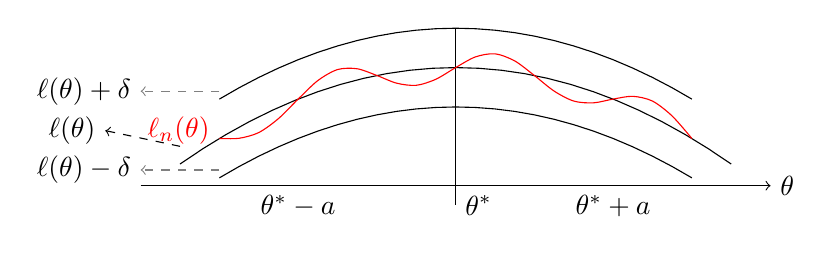
\begin{tikzpicture}
  \draw[->] (-4,0) -- (4,0) node[right] {$\theta$};
  \draw (0,2) -- (0,-.25) node[right] {$\theta^*$};
  \draw node[below] at (-2,0) {$\theta^* - a$}; 
  \draw node[below] at ( 2,0) {$\theta^* + a$}; 
  \draw plot[domain=-3:3] ({\x}, {-0.1*(\x*\x)+2}) node[right,black] {};
  \draw plot[domain=-3.5:3.5] ({\x}, {-0.1*(\x*\x)+(1.5)}) 
    node[right,black] {};
  \draw plot[domain=-3:3] ({\x}, {-0.1*(\x*\x)+1}) node[right,black] {};
  \draw[gray,dashed,->] (-3,0.2) -- (-4,0.2) 
       node[left,black] {$\ell(\theta) - \delta$};
  \draw[gray,dashed,->] (-3,1.2) -- (-4,1.2) 
       node[left,black] {$\ell(\theta) + \delta$};
  \draw[red,domain=3:-3,smooth] plot (\x, {-0.1*(\x*\x)+(1.5)+0.2*sin(3.14159*\x r)});
  \draw node[red,left] at (-3,0.7) {$\ell_n (\theta)$};
  \draw[->,dashed] (-3.5,0.5) -- (-4.45, 0.7) 
       node[black,left] {$\ell(\theta)$};
\end{tikzpicture}   
\end{figure}
We know that $\ell_n(\theta) \overset{P}{\longrightarrow} \ell(\theta)$ by WLLN.
Further, \href{http://www.amazon.com/Course-Sample-Chapman-Statistical-Science/dp/0412043718}{Ferguson (1996)}, this holds uniformly in $\theta$ for
\[
| \theta - \theta^*| \leq a.
\]
Hence for all $\delta > 0$,
\[
\Pr\left( \max_{|\theta - \theta^*| \leq a} \bigg|\ell_n(\theta) - \ell(\theta)\bigg| > \delta \right) \overset{n \uparrow \infty}{\longrightarrow} 0.
\]

Does this imply that $\hat \theta_n = \argmax_{|\theta - \theta^*| \leq a} \ell_n(\theta) \overset{P}{\longrightarrow} \theta^*$?
Yes! \href{http://projecteuclid.org/euclid.aoms/1177729952}{Wald (1948)}.

% \paragraph{Asymptotic Distribution of MLE}
% What about the asymptotic distribution of MLE? Let $\hat \theta_n = \theta^* + \frac{Z_n}{\sqrt n}$, i.e. $Z_n = \sqrt n (\hat \theta_n - \theta^*)$.

% \begin{theorem}   $Z_n \overset{\mathcal D}{\longrightarrow} \mathcal N \left(0, \frac{1}{I(\theta^*)}\right)$. \end{theorem}
% Note that $\hat \theta_n$ is \emph{not} a summation, it's a max.
% How can we apply CLT?

% \paragraph{Delta Method} Start with $\ell'_n(\hat \theta_n) = 0$, which
% is a fact we derived. We also know that $\ell'(\theta^*)=0$.\hl{Why}
% We may rewrite this as
% \[
% 0 = \ell'_n(\hat \theta_n) = \ell'_n(\theta^* + \frac{Z_n}{\sqrt n}) = \ell_n'(\theta^*) + \ell''_n(\tilde{\theta}_n) \frac{Z_n}{\sqrt n},
% \]
% for $\tilde{\theta_n}$ between $\theta^*$ and $\hat \theta_n$. Hence
% by consistency, $\tilde{ \theta_n} \overset{P}{\longrightarrow} \theta^*$.

% Now, we solve for $Z_n$, yielding

% \[
% Z_n = \frac{\sqrt n \ell'_n(\theta^*)}{- \ell_n''(\tilde{\theta_n})},
% \] 
% where
% \[
% \ell_n'(\theta^*) = \frac{1}{n} \sum_{j=1}^n \frac{f'(x_j|\theta^*)}{f(x_j|\theta^*)}.
% \]

% Since $\Bbb E [ \ell'(\theta)] = 0$, then $\textrm{var}(\ell'(\theta)) = I(\theta)$. (\hl{no star?}) So,

% \[
% \sqrt n (\ell_n'(\theta^*) \overset{\mathcal D}{\longrightarrow} \mathcal N (0, I(\theta^*),
% \]
% and
% \[
% \ell''(\theta) = \frac{1}{n}\sum_{j=1}^n \left( \frac{f''(x_j|\theta^*)}{f(x_j|\theta^*)} - \frac{(f'(x_j|\theta^*))^2}{f^2(x_j|\theta^*)}\right) \overset{\textrm{WLLN}}{\longrightarrow} - I(\theta^*).
% \]

% Hence by \emph{Slutsky}'s theorem,
% \[
% Z_n = \frac{\sqrt n \ell_n'(\theta^*)}{-\ell''_n(\tilde \theta_n)} \overset{\mathcal D}{\longrightarrow} \frac{1}{I} \mathcal{N} (0,I) = \mathcal N (0, \frac{1}{I}).
% \]

% \section{Properties of Estimators}
% We cover several finite sample properties of estimators before delving into % their asymptotic properties.
% \subsection{Finite sample properties}
% We define the \emph{bias} of an estimator $\hat \theta$ as
% \[
% \textrm{Bias}_\theta\left(\hat \theta \right) = \mathbb E[\hat \theta ] - \theta.
% \]


% \subsection{Asymptotic properties} 
% An estimator $\hat \theta_n$ is consistent if $\hat \theta_n \overset{P}{\longrightarrow} \theta$
% for all $\theta \in\ Theta$.

\section{Statistical Inference}
Lastly, we investigate the cornerstone of statistical inference: the hypothesis test. \subsection{Hypothesis testing} \subsection{Confidence intervals}

\section{Homework/Practice}
 \section*{Problem \#1}  \paragraph{Question} A target is made of 3 concentric circles of radii $1/\sqrt{3}$, 1, and $\sqrt{3}$ feet. Shots within the inner circle are given 4 points, shots within the next ring are given 3 points, and shots within the third ring are given 2 points. Shouts outside the target are given 0 points.  Let $X$ denote the distance of the hit from the center (in feet), and let the p.d.f. of $X$ be  \[ f(x) = \frac{2}{\pi (1 + x^2)} \boldsymbol{1}\{x > 0\} \]  What is the expected value of the score of a single shot?  \paragraph{Solution} Using the definition of the expectation of a discrete-valued random variable, we have that  \begin{align*} \mathbb E[\text{single shot}] &= \sum_{x \in X} x \cdot \Pr(X = x) \\  &= 0 \cdot \Pr(X > \sqrt{3}) + 2 \cdot \Pr(1 < X < \sqrt{3}) + 3 \cdot \Pr(\frac{1}{\sqrt{2}} < X < 1) + 4 \cdot \Pr(X < \frac{1}{\sqrt{3}}) \end{align*}  The solution is simple once we solve for the c.d.f. of our random variable $X$. By definition,  \[ F(x) = \int_0^x f(x) dx = \int_0^x \frac{2}{\pi(1 + x^2)} dx \]  Recall that when $\sin \theta$ and $\cos \theta$ are defined using a unit circle, the $(x,y)$ point which lay on the unit circle is given by $(\cos \theta, \sin \theta)$, where $\theta$ denotes the angle from the origin.  Therefore, by the Pythagorean theorem, we have the identity that $\sin^2 \theta + \cos^2 \theta = 1$, since we can describe any point on the unit circle by a (possible degenerate) right triangle. We may then derive that  \begin{align*} \sin^2 \theta + \cos^2 \theta &= 1 \\ \frac{\sin^2 \theta}{\cos^2 \theta} + \frac{\cos^2\theta}{\cos^2 \theta} &= \frac{1}{\cos^2 \theta} \\ \tan^2 \theta + 1 &= \sec^2 \theta \end{align*}  This informs how we may use $u$-substitution to solve for our c.d.f. Let $x = \tan \theta$. Then,  \begin{align*} \frac{d}{d \theta} \tan \theta &= \frac{d}{d \theta} \frac{\sin \theta}{\cos \theta} \\  &= \frac{d}{d \theta} \sin \theta \cos^{-1} \theta \\  &= \frac{\cos \theta}{\cos \theta} + \frac{-\sin \theta}{\cos^2 \theta} \cdot (-\sin \theta) \\  &= \frac{\cos^2 \theta + \sin^2 \theta}{\cos^2 \theta} \\ &= \frac{1}{\cos^2 \theta} \\ &= \sec^2 \theta \end{align*}  If $x = \tan \theta$, then $\theta = \arctan x$, and further  \[ \frac{dx}{d\theta} = \sec^2 \theta \implies dx = \sec^2 \theta d \theta. \]  This is great because we can use $u$-substitution to reduce our integral to something very simple:  \[ \int \frac{1}{1 + x^2}dx = \int \frac{1}{\sec^2 \theta} \sec^2 \theta d\theta = \int d \theta = \theta + C \]  Therefore,  \begin{align*} \frac{2}{\pi} \int_0^x  \frac{1}{1+x^2}dx &= \frac{2}{\pi} \arctan x \bigg |_0^x = \frac{2}{\pi} \arctan x \end{align*}  Note that $\arctan 0 = 0$ and  $\underset{x \to \infty}{\lim} \arctan x \to \pi/2$, so that  $F(0) = 0$ and $\underset{x \to \infty}{\lim} F(x) \to 1$, which is how we expect our c.d.f. to behave for this random variable.  Now,  \begin{align*} \mathbb{E}[\text{single shot}] &= \sum_{x \in X} x \cdot \Pr(X = x) \\  &= 0 \cdot \Pr(X > \sqrt{3}) + 2 \cdot \Pr(1 < X < \sqrt{3}) + 3 \cdot \Pr(\frac{1}{\sqrt{2}} < X < 1) + 4 \cdot \Pr(X < \frac{1}{\sqrt{3}}) \\ &= 2 \bigg( F(\sqrt{3}) - F(1) \bigg) + 3 \bigg(F(1) - F(1/\sqrt{3}) \bigg) + 4 F(1/\sqrt{3}) \\ &\approx 3.403  \end{align*}  \section*{Problem \#2}   \paragraph{Question} Assume that the random variable $X$ has the exponential distribution  \[ f(x|\theta) = \theta e^{-\theta x} \boldsymbol{1}\{x > 0, \theta > 0\} \]  where $\theta$ is the parameter of the distribution. Use the method of maximum likelihood to estimate $\theta$ is 5 observations of $X$ are $x_1 = 0.9$, $x_2 = 1.7$, $x_3 = 0.4$, $x_4 = 0.3$, and $x_5 = 2.4$ are generated independent and identically distributed.  \paragraph{Answer} We are told that  \[ x_1, \ldots, x_n \overset{i.i.d.}{\sim} \textrm{exp} (\theta) \]  By independence, we have that  \[ f(x_1, \ldots, x_n | \theta_1, \ldots, \theta_n) = \prod_{i=1}^n f(x_i|\theta_i) \]  and by identically distributed, we have that  \[ \prod_{i=1}^n f(x_i) = \theta e^{-\theta x_i} \]  Therefore,  \[ f(x_1, \ldots, x_n|\theta) = \prod_{i=1}^n \theta e^{- \theta x_i} = \theta^n e^{-\theta \sum_i x_i} \]  Our likelihood function is given by  \[ L(\theta|x_1, \ldots, x_n) = \theta^n e^{-\theta \sum_i x_i}. \]  Maximizing a monotonic increasing transformation of the likelihood is the same as maximizing the likelihood, so to make life easier we take the log-likelihood:  \[ \lg L(\theta|x_1, \ldots, x_n) = n \lg \theta - \theta \sum_i x_i \]  Maximizing this by taking the derivative and setting it to zero shows that   \begin{align*} \frac{d}{d \theta} \lg L(\theta |x_1, \ldots, x_n) = \frac{n}{\theta} - \sum_i x_i &= 0 \\ \frac{n}{\theta} &= \sum_i x_i \\ \implies \hat{\theta}_{\text{mle}} &= \frac{n}{\sum_i x_i} \end{align*}  In other words, our maximum likelihood estimator for our parameter $\theta$ is simply the reciprocal of the sample mean. Note that we can convince ourselves that we have found a true maximum by taking the second derivative of our likelihood function and checking that it is concave, yielding  $\frac{d}{d \theta} \frac{n}{\theta} - \sum_i x_i = \frac{-n}{\theta^2}$, which is an upside down parabola and therefore has a single maximum point.  If $x = (0.9, 1.7, 0.4, 0.3, 2.4)$, then $\sum_i x_i = 5.7$, and $\bar{x} = 57/50 = 1.14$. Therefore, we see that  \[ \hat{\theta}_{\text{mle}} = \frac{1}{\bar{x}} = \frac{1}{1.14} \approx 0.877. \] 

\bibliographystyle{plain}
\begin{thebibliography}{10}
\bibitem{clain: ec2120}
G. Chamberlain.
\newblock {\em Econometrics 2120}.
\newblock Harvard University, Winter 2017.

\bibitem{papa: 308}
G. Papanicalou.
\newblock {\em CME 308: Stochastic Processes}.
\newblock Stanford University, Spring 2016.

\bibitem{ferguson: lst}
Thomas S. Ferguson
\newblock {\em A course in large sample theory}.
\newblock University of California, Los Angeles.

\bibitem{Wald: 48}
Abraham Wald.
\newblock {\em Note on the consistency of the maximum likelihood estimate}.
\newblock Annals of Mathematical Statistics, 1949.

\end{thebibliography}
  \end{document}